\chapter{Conclusion}
\label{chap:conclusion}

In conclusion, the implementation of a Python routine for complete automation and integration of the system has improved the precision of experiments and enabled real-time collection of extensive data without requiring the expertise and time of a specialized scientist. 
This project underscores the potential of automation in enhancing scientific research and accelerating progress towards achieving research goals.
In addition to its potential in scientific research, the software developed in this project can also be leveraged by industrial approaches. 
Furthermore, the classification methods and system control implemented in this project have yielded promising results and can be further optimized in the future. Overall, this project serves as a contribution towards the advancement of automated systems and the optimization of experimental processes.

\section{Proposal for continuing}

To continue, my proposal would be to prioritize the improvement of the classification step. 
Ideally, we could use machine learning or another algorithm to ensure accurate classification of individual data samples.

By achieving a reliable classification, we can then implement more effective controller logic or approaches. 
In this regard, I would like to present the concept of a fuzzy controller as a potential solution.

To finish, I would propose a final investment in the system portability so that it can be applicable in remote applications.

\subsection{Machine Learning}

\subsection{Fuzzy Controller}

        One challenge in implementing the controller is that we do not have continuous feedback. 
        Instead, the feedback from the controller loop is a classification, which makes it difficult to apply many of the principles of control theory that are designed for continuous control. 
        As this project involves logical control, it requires a different approach. 
        
        The fuzzy approach is an attempt to quantify the classification and fit different control models.

        For that, I fuzzyfied the controller input with the data acquired in an experiment of step routine\ref{subsec:step_routine}. With the data, I mapped the area of each spraying mode according to its potential as shown in the Figure \ref{fig:fuzzy_input}.
        Figures \ref{fig:Fuzzyfication} and \ref{fig:defuzzyfication} shows the steps of fuzzyfication and defuzzyfication between the input and output of the controller.

        \begin{multicols}{2}

            \begin{figure}[H]
                \centering
                \resizebox{90mm}{!}{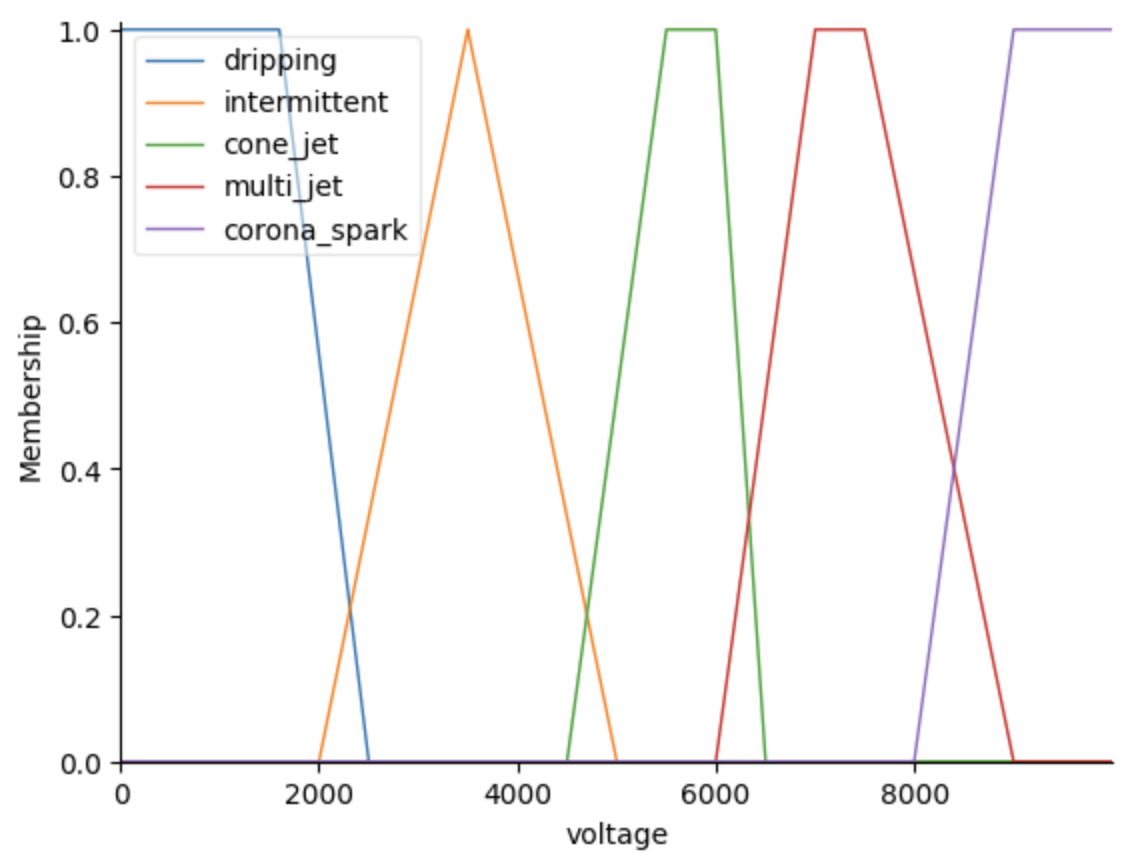
\includegraphics{Figuras/fuzzy/fuzzyfy_input.png}}
                \caption{Fuzzyfication of the voltage input}
                \label{fig:fuzzy_input}
            \end{figure}

            \begin{figure}[H]
                \centering
                \resizebox{90mm}{!}{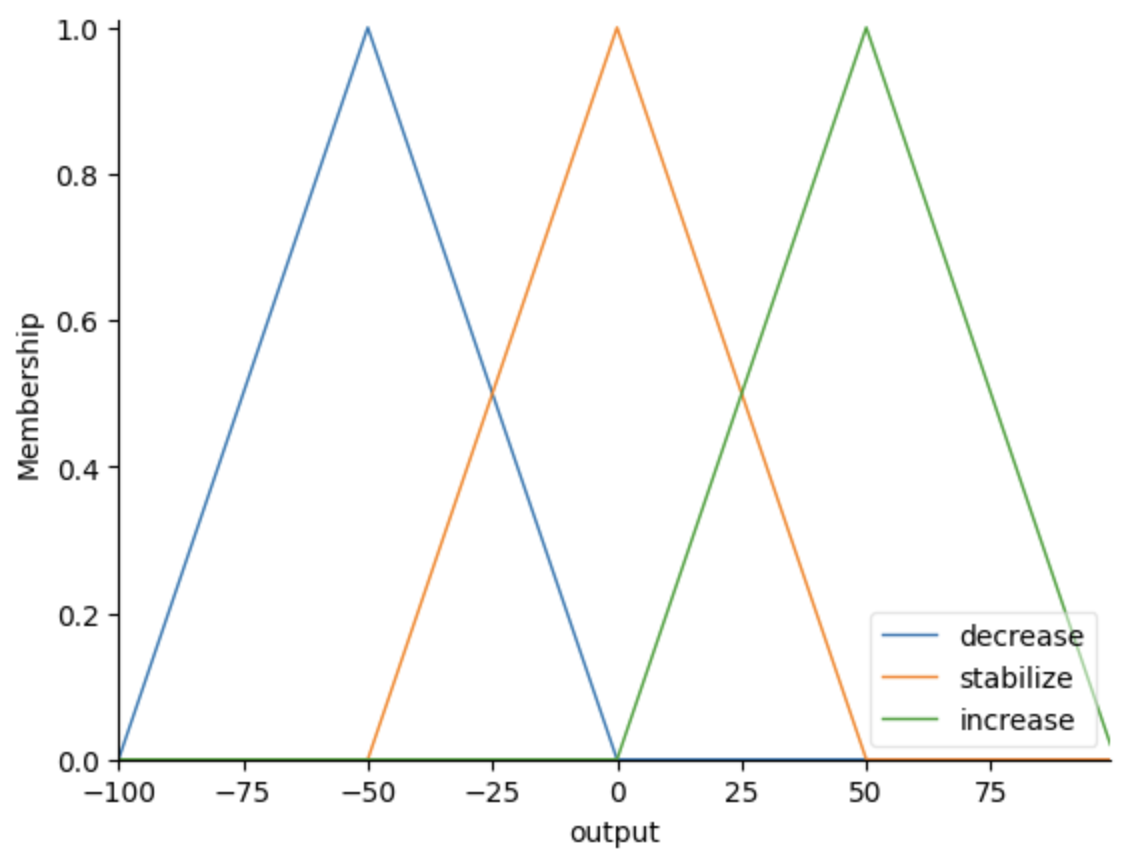
\includegraphics{Figuras/fuzzy/defuzzyfy.png}}
                \caption{Defuzzyfication of output}
                \label{fig:fuzzy_output}
            \end{figure}

        \end{multicols}


        Our controller is a machine that calculate the output with a geometrical calculus on the membership functions of the input and output according to our rules.
        The rules are listed below.

        Fuzzy Rules:

        -> IF dripping THEN increase

        -> IF intermittent THEN increase

        -> IF cone jet THEN stabilize

        -> IF multi jet THEN decrease

        -> IF corona THEN decrease


        % \begin{figure}[H]
        %     \centering
        %     \resizebox{80mm}{!}{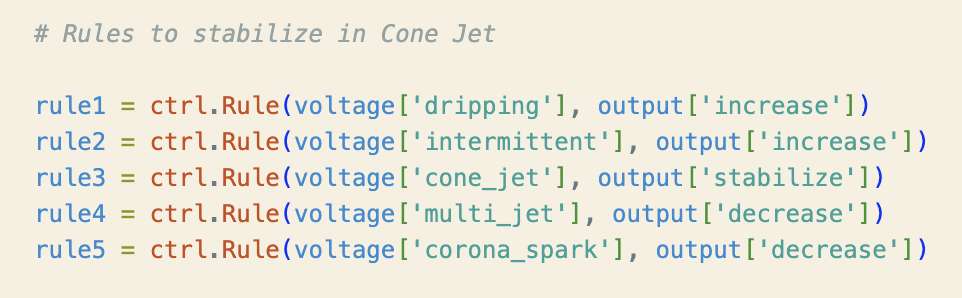
\includegraphics{Figuras/fuzzy/rules.png}}
        %     \caption{Fuzzy Rules}
        %     \label{fig:fuzzy_rules}
        % \end{figure}

        For testing the concept I've showed two possible states where the voltage is below the necessary to stabilize in cone jet and when is above that voltage. We can see in figures \ref{fig:fuzzy_test1} and \ref{fig:fuzzy_test2} that each test the output was either increase or decrease the actuator signal.
        
        \begin{multicols}{2}
            
            \begin{figure}[H]
                \centering
                \resizebox{90mm}{!}{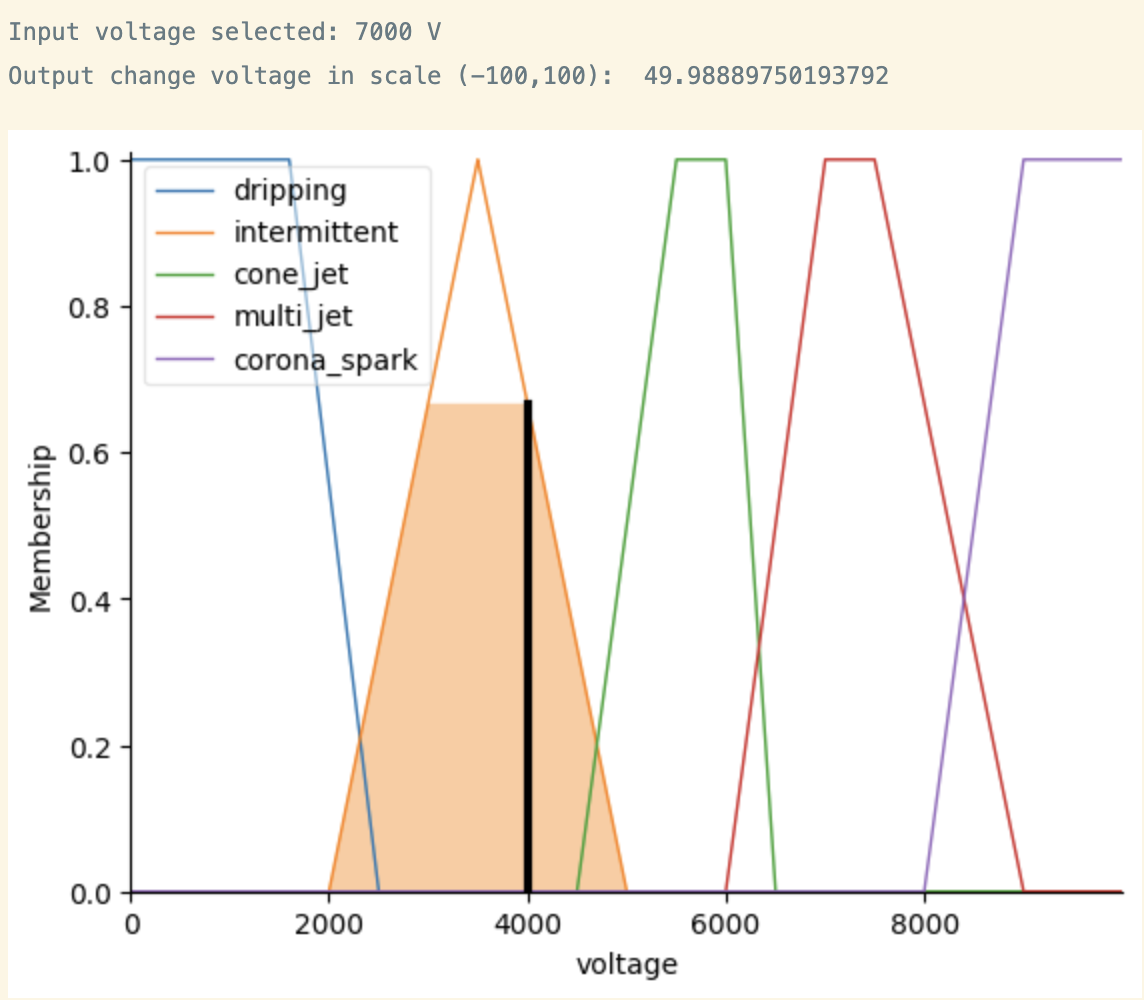
\includegraphics{Figuras/fuzzy/test2.png}}
                \caption{Test 1: fuzzy controller. Input voltage 4000 V the controller output to increase the voltage.}
                \label{fig:fuzzy_test2}
            \end{figure}
            
            \begin{figure}[H]
                \centering
                \resizebox{90mm}{!}{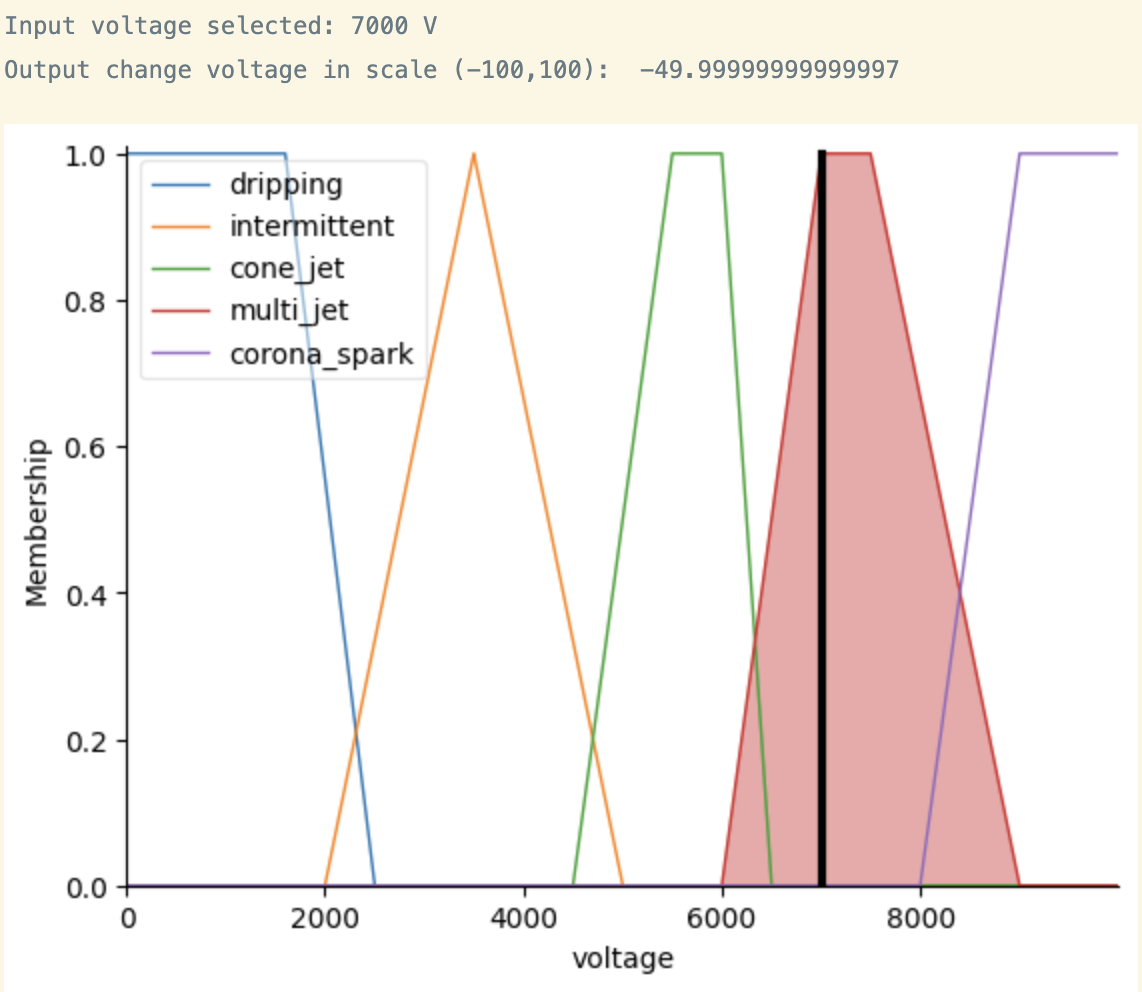
\includegraphics{Figuras/fuzzy/test1.png}}
                \caption{Test 2: fuzzy controller. Input voltage 7000 V the controller output to decrease the voltage.}
                \label{fig:fuzzy_test1}
            \end{figure}
            
        \end{multicols}
        
        Note that, for this method to work it is needed to run a step sequence to scan the cone jet stability island. With that data, create the input membership function. Then, run the controller routine in fuzzy mode.

    
    \subsection{System Portability}
    \label{subsec:portability}

        Raspberry Pi


    \section{Final Discussions}

        The works therefore presented here are a continuation and optimization of the routine to make it more precise and applicable to both industrial and research approaches.
        The previous student work was focused in predicting corona streamers or spark discharges, therefore her automation routine was a first version concept that proved to be valuable.
        From the development done by me, it highlights the results:
        
        - Integrate liquid pump to the software and developed a routine with it.
        
        - Modeled the software to fit a control model turning it easy to implement new control algorithms or experiment routines.
        
        - Remodel the software to support threads in order to separate each subsystem and exchange data between them with use of queues data structures.
        
        - Developed a classification for multi jet spraying mode.
        
        - Developed a simple controller to proof the concept.
        
        - Optimize the saving of data to a real time streaming together with more sensors' data.
        
        - Restructured algorithm usability in order to make it more intuitive with the setup file.
        
        
\clearpage
